%\documentclass[margin=0mm]{standalone}
%\usepackage{tikz}
%\usepackage{pgfplots}
% \pgfplotsset{compat=newest}
%
%
%\usepackage{currfile,hyperxmp}
%\usetikzlibrary{math,matrix,fit,positioning}
%\usepgfplotslibrary{groupplots}
%
%
%\begin{document}

  

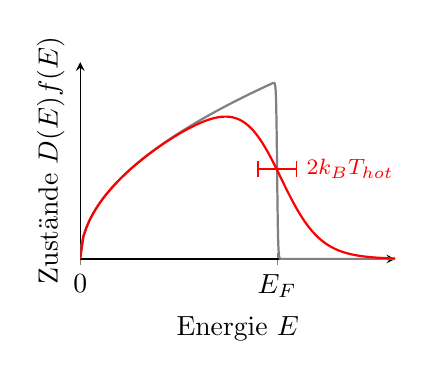
\begin{tikzpicture}
%\useasboundingbox (-1.0,-1.0) rectangle (10.2,4.2);
%\draw (-1,-1.0) rectangle (10.2,4.2);
%

 
\begin{axis}[
    height=2.5cm,
    width=4cm,
    xtick pos = bottom,
    scale only axis,
            separate axis lines,
  axis x line=bottom,
  axis x line shift=0pt,
  %xlabel shift=10pt,
  axis y line=left,
  axis y line shift=0pt,
%  ylabel shift=10pt      
  axis y line=left, clip=true,
  ymin = 0, ymax = 3.5,
%  ytick = \empty,
%  xtick = {-3,-2, -1, 0,1,2,3},
%,ytick pos = left, ytick = {0}, 
% xmin=1320, xmax = 1520, xtick = {1415}, xticklabel = {1415}
 ylabel = {Zustände $D(E) f(E)$}, xlabel = {Energie $E$},
 ytick = \empty, yticklabel = \empty,
 xtick = {0, 10},
 xticklabels = {0, $E_F$},
%ylabel = {extinktion}, xlabel = {energy (eV)},
%ytick pos = left, 
 xmin=0, xmax = 16,
 ]
\
%\addplot[blue,thick, domain= -4:-8, samples=100]{ 1/ (exp(x) + 1)  - 0.15* exp(- (x+6)^2 / 0.25) };
%\addplot[blue, thick,domain= 4:8, samples=100]{   1/ (exp(x) + 1)  +  0.15* exp(- (x-6)^2 / 0.25)) };
\addplot[gray, thick, domain=0:16, samples=2000]{sqrt(x) / (exp( (x-10)/0.025) + 1)};

\addplot[red, thick,domain=0:16, samples=100]{sqrt(x) / (exp((x-10)/1) + 1)};

\draw[|-|,red] (9, 1.6) -- (11, 1.6) node[right] {\footnotesize $2 k_B T_{hot}$};
%\draw[|-|] (-2, 0.4) -- (2, 0.4) node[right] {\footnotesize $k_B T_{hot}$};

%\draw[|-|] (-6, -0.03) node[left] {\footnotesize $h \nu$} -- (6, -0.03) ;

\end{axis}


\end{tikzpicture}

%\end{document}